%==============================================================================
% Section 4: Spin-2 Sector: Full Shear Completion and Geometric Phase Structure
%==============================================================================
\section{Spin-2 Sector: Full Shear Completion and Geometric Phase Structure}
\label{sec:spin2}

This section completes the squash/shear deformations as the full shear tensor
and presents the final phase diagram of the spin-2 quintet.  The conclusions are:
five-fold degeneracy at the isotropic point; softening of the $m=0$ singlet on
the positive-$\varepsilon$ side; and a second-order phase transition of the
$m=\pm 2$ sector on the negative-$\varepsilon$ side.

\subsection{Full Shear Tensor as the Spin-2 Quintet}

A description in terms of raw geometric variables $(\varepsilon,s,\phi)$ is
useful for following a particular slice but insufficient to represent the entire
spin-2 sector.  We adopt
\begin{equation}
  h_{ij} = \sum_{A=1}^5 q_A\,(T_A)_{ij}
\end{equation}
and treat the five components of $\Sym_0^2(\mathbb{R}^3)$ as a complete spin-2
quintet.  Here $q_A$ are the final variables aligned with the $SO(3)$ irreducible
basis; $\varepsilon$ and $s$ are used as projections of $q_A$ onto specific
directions.

\begin{figure}[H]
  \centering
  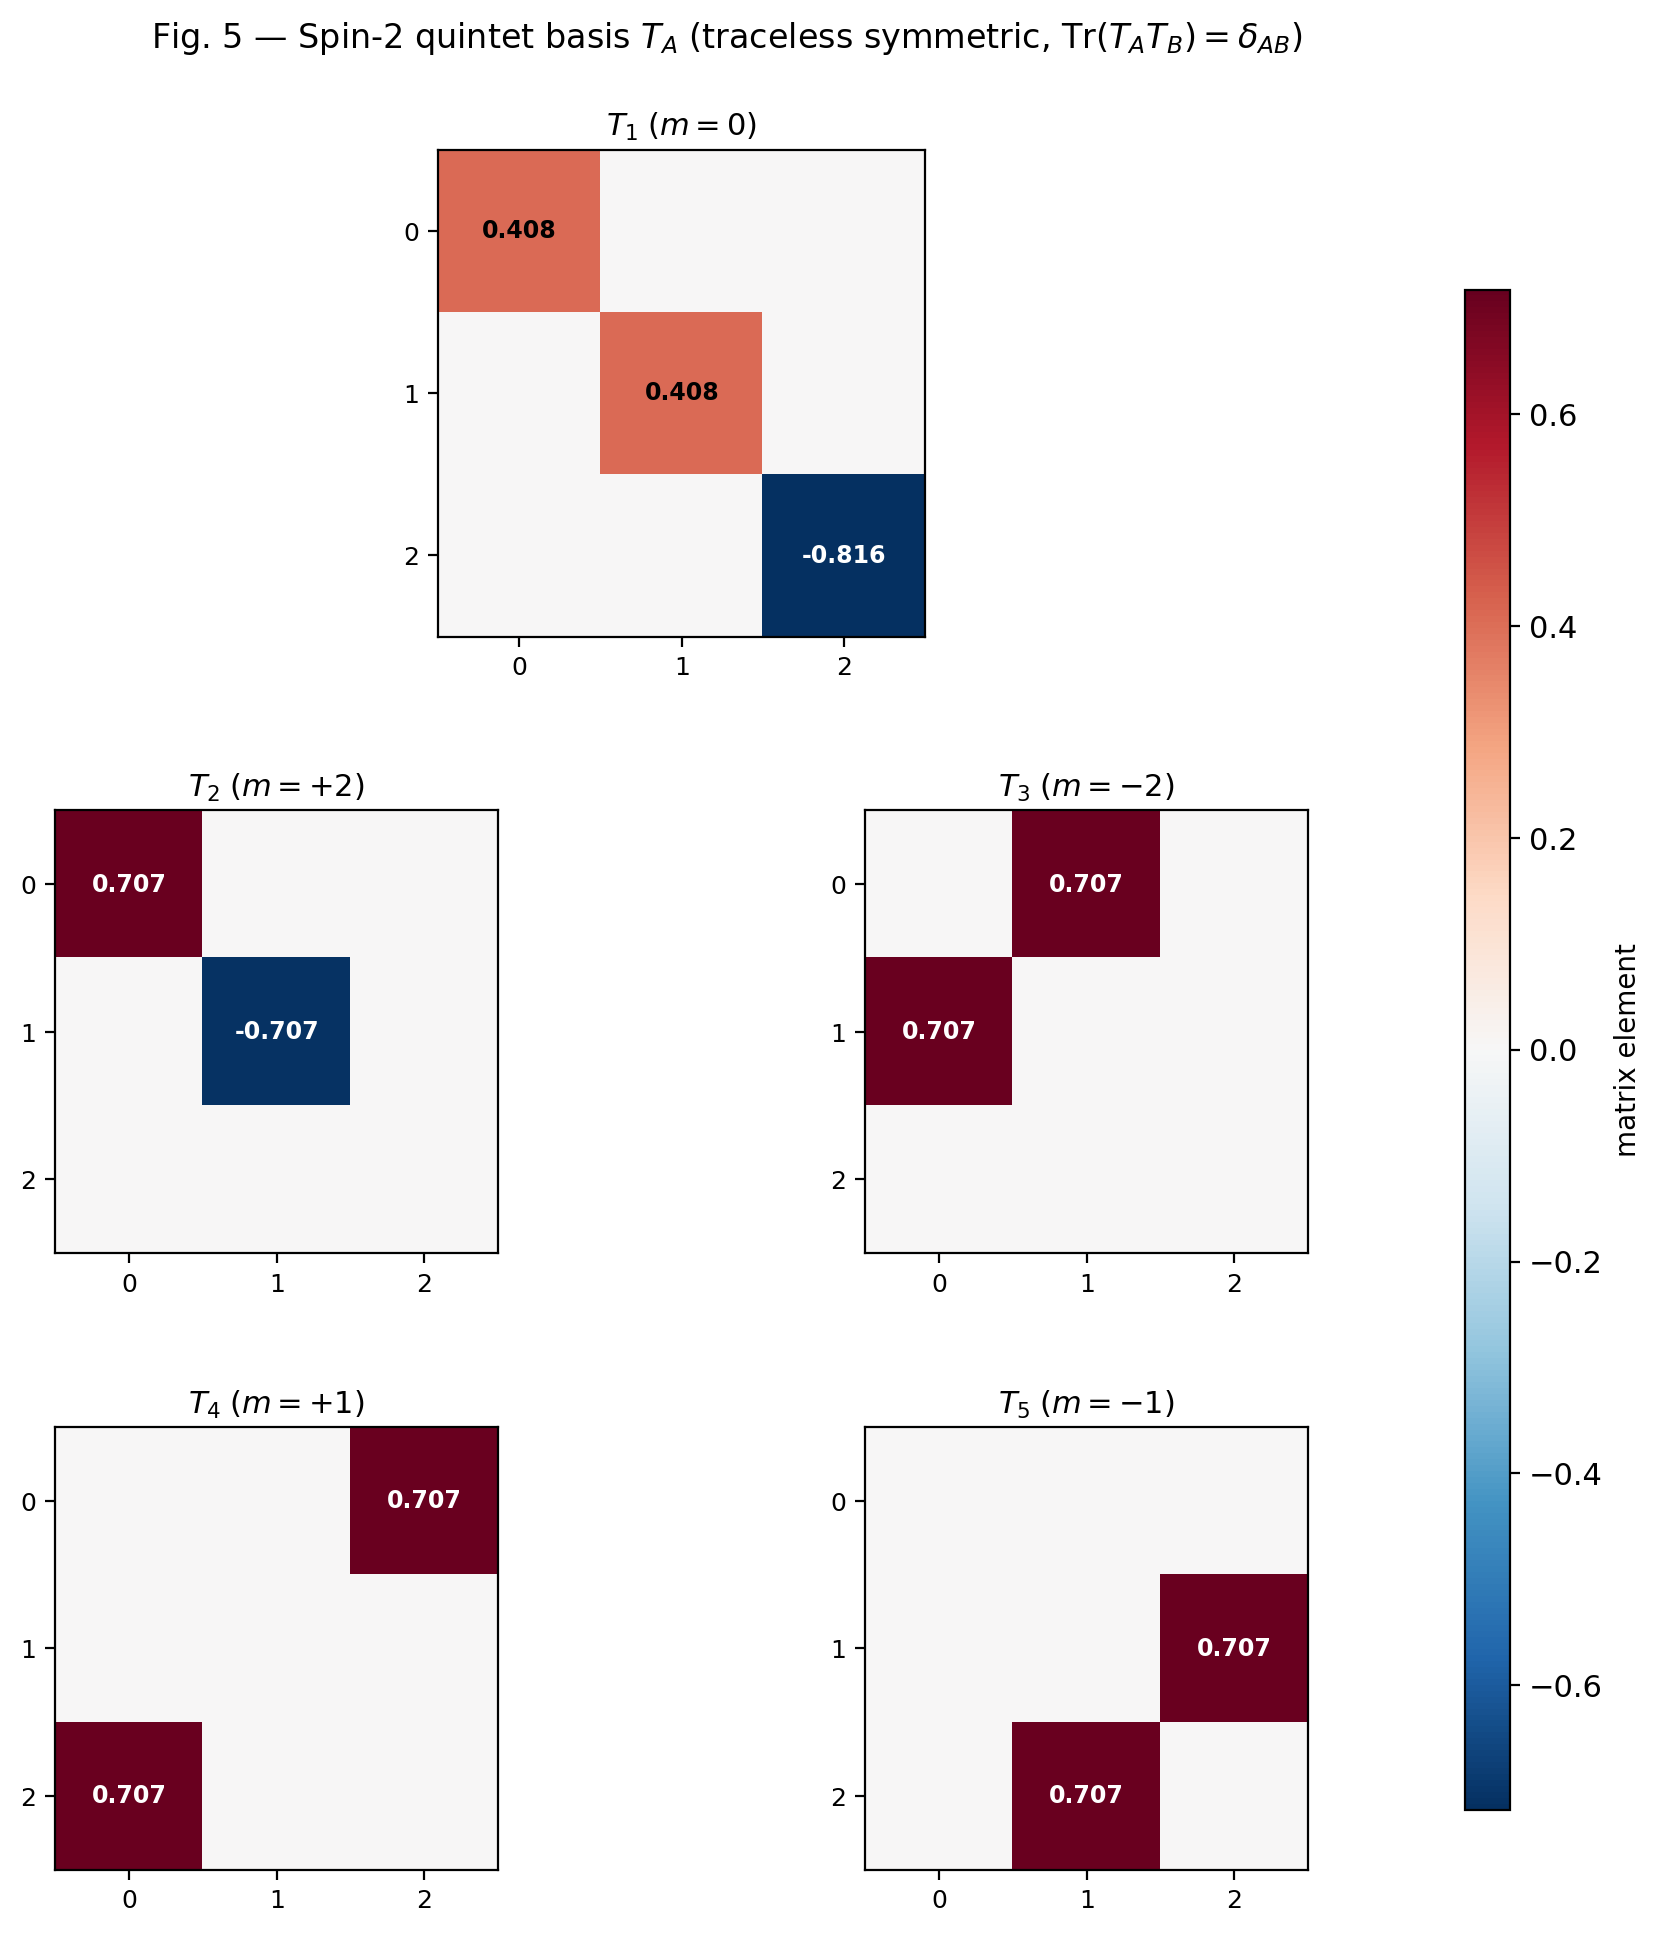
\includegraphics[width=0.72\textwidth]{figures/fig05_TA_basis.png}
  \caption{Basis vectors $T_1,\ldots,T_5$ of the spin-2 quintet
           $\Sym_0^2(\mathbb{R}^3)$.  The three sectors correspond to the
           residual $SO(2)$ representations $m=0$, $m=\pm 2$, and $m=\pm 1$.}
  \label{fig:TA_basis}
\end{figure}

\subsection{Isotropic Point and Schur Degeneracy}

At the isotropic point the residual symmetry is the full $SO(3)$, so the spin-2
Hessian is proportional to the identity matrix on each irreducible representation.
Consequently,
\begin{equation}
  \Veff = V_0 + \lambda\,\tr(h^2) + O(|q|^3)
        = V_0 + \lambda\sum_{A=1}^5 q_A^2 + O(|q|^3),
\end{equation}
giving
\begin{equation}
  H_{AB} = \left.\frac{\partial^2 V}{\partial q_A \partial q_B}\right|_0
          = 2\lambda\,\delta_{AB}.
\end{equation}
The generalised mass is equal for all five components:
\begin{equation}
  \mu_q^2 = 48\pi^2.
\end{equation}
This is the spin-2 sector's Schur degeneracy.

\begin{figure}[H]
  \centering
  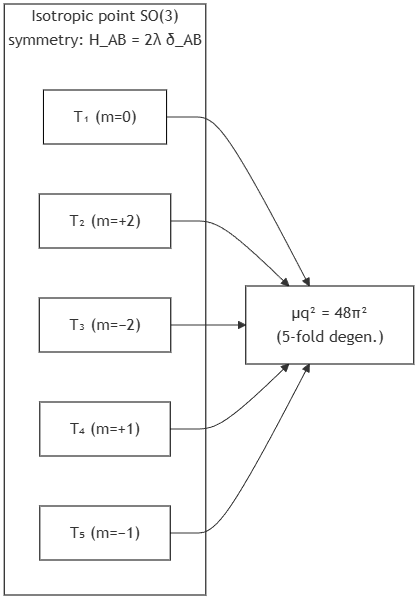
\includegraphics[width=0.6\textwidth]{figures/fig06_five-fold_degeneracy.png}
  \caption{Five-fold degeneracy of the spin-2 quintet at the isotropic point.
           Schur's lemma $H_{AB}=2\lambda\delta_{AB}$ enforces equal mass
           $\mu_q^2=48\pi^2$ for all five components.}
  \label{fig:schur}
\end{figure}

\subsection{$SO(3)$ to $SO(2)$ Splitting under Squash Background}

Under a positive-$\varepsilon$ squash background the symmetry reduces to
$SO(3)\to SO(2)$, and the spin-2 quintet splits as follows.

\begin{table}[H]
\centering
\begin{tabular}{lll}
\toprule
Residual charge & Basis & Interpretation \\
\midrule
$m=0$     & $T_1$          & squash singlet \\
$m=\pm 2$ & $(T_2, T_3)$   & in-plane doublet \\
$m=\pm 1$ & $(T_4, T_5)$   & off-axis doublet \\
\bottomrule
\end{tabular}
\caption{Residual $SO(2)$ decomposition of the spin-2 quintet under a
         positive-$\varepsilon$ squash background.}
\label{tab:SO2split}
\end{table}

The key observation is that the order in which soft modes appear is organised by
these residual representations.

\begin{figure}[H]
  \centering
  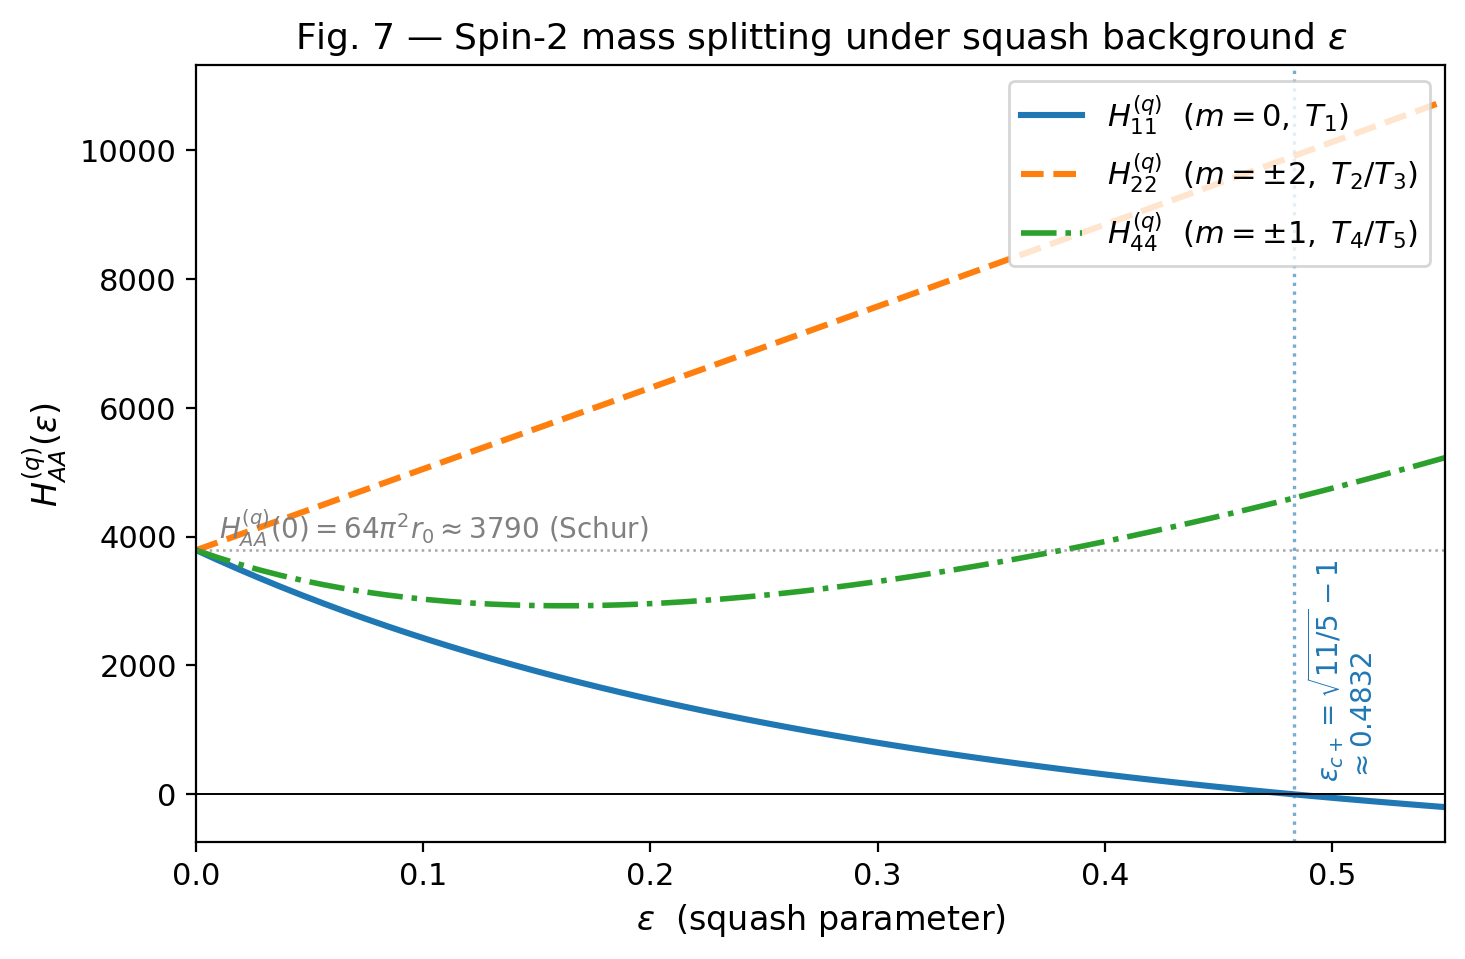
\includegraphics[width=0.75\textwidth]{figures/fig07_spin2_splitting.png}
  \caption{Mass splitting of the spin-2 quintet as a function of the squash
           parameter $\varepsilon$.  The three branches correspond to $m=0$
           (singlet $T_1$), $m=\pm 2$ (doublet $T_2,T_3$), and $m=\pm 1$
           (doublet $T_4,T_5$).  The $m=0$ branch reaches zero first at
           $\varepsilon_{c+}$.}
  \label{fig:spin2_split}
\end{figure}

\subsection{Positive-$\varepsilon$ Side: First Soft Mode}

From the full shear analysis, on the positive side the $T_1$ singlet becomes
soft first.  The critical value is
\begin{equation}
  \varepsilon_{c+} = \sqrt{\frac{11}{5}} - 1 \approx 0.48324,
  \qquad
  r_0(\varepsilon_{c+}) \approx 2.8114,
\end{equation}
at which $\mu_\varepsilon^2\to 0$.

\begin{figure}[H]
  \centering
  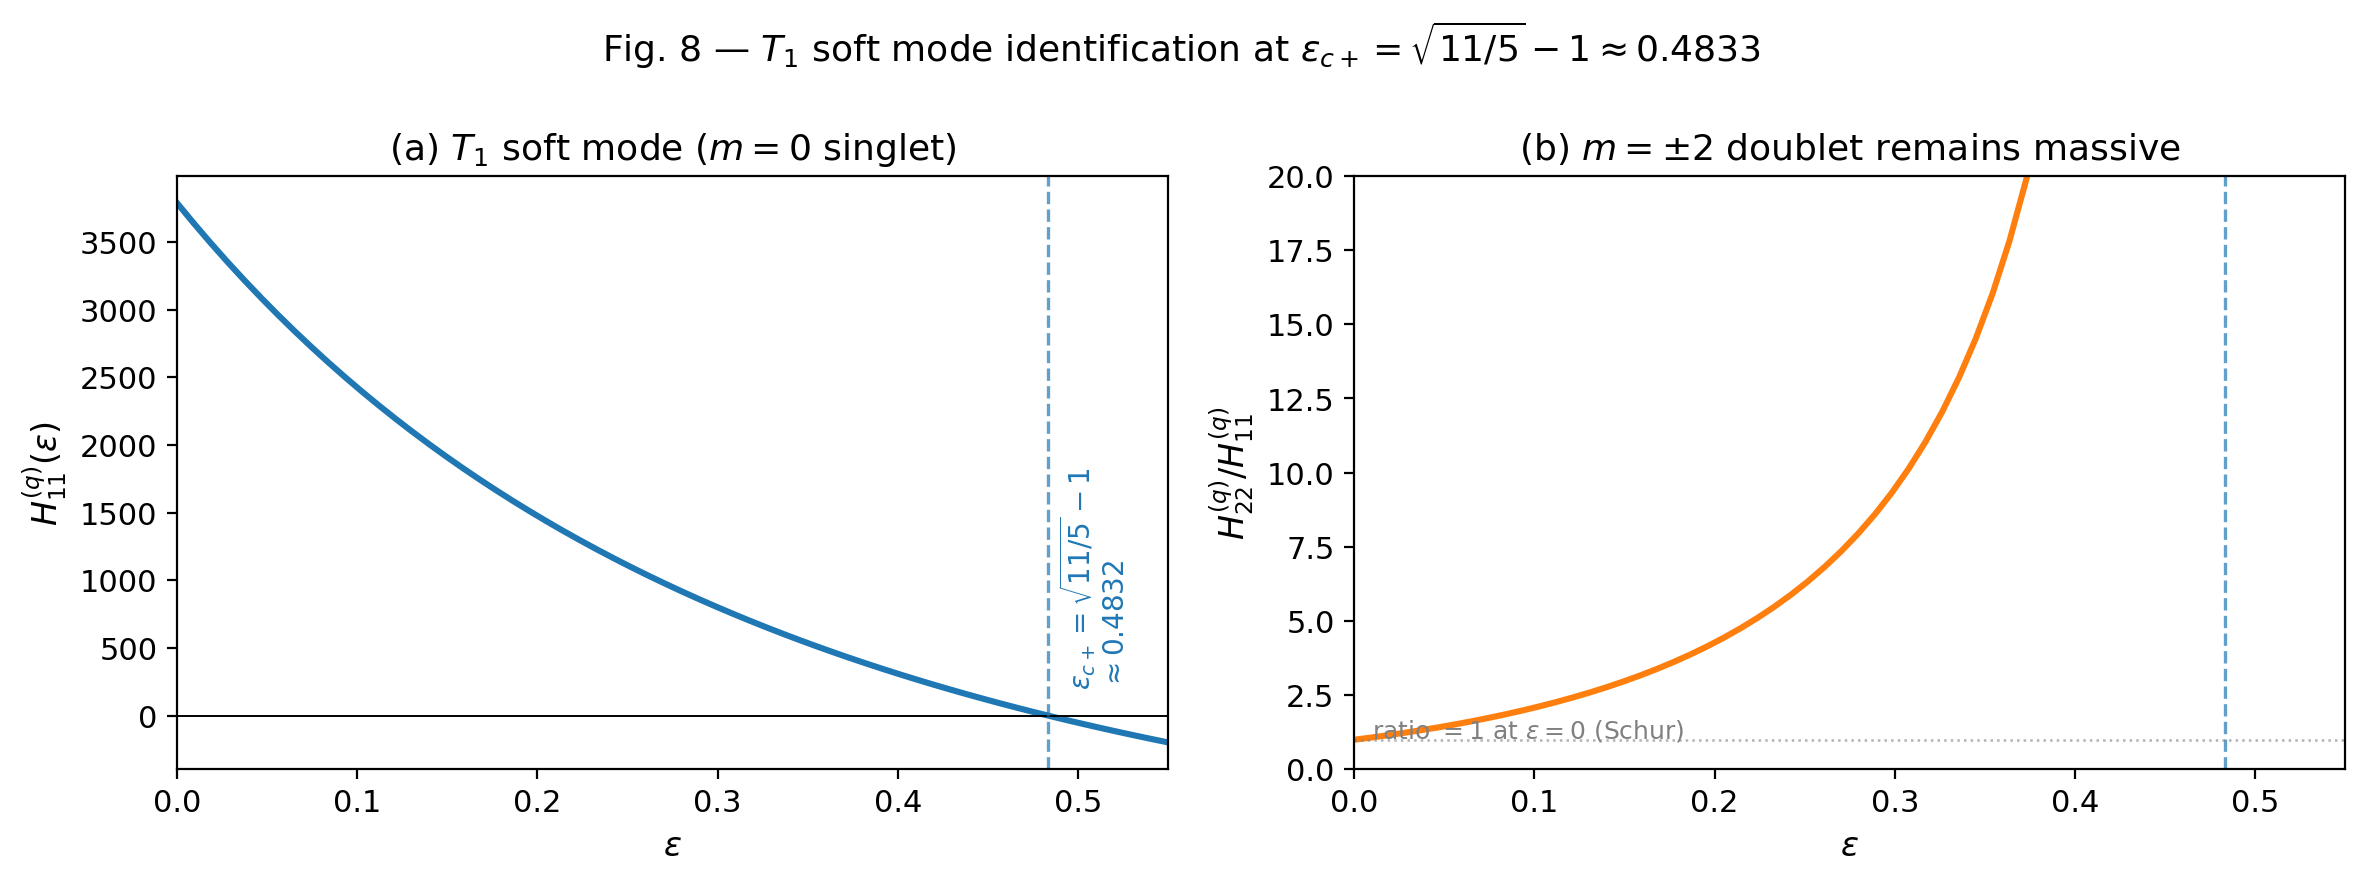
\includegraphics[width=0.85\textwidth]{figures/fig08_soft_mode.png}
  \caption{Softening of the $m=0$ mode $\mu_\varepsilon^2(\varepsilon)$ on the
           positive-$\varepsilon$ side.  The curve reaches zero at the exact
           critical point $\varepsilon_{c+}=\sqrt{11/5}-1\approx 0.483$, while
           the $m=\pm 2$ branch remains massive.}
  \label{fig:soft_mode}
\end{figure}

Key points to emphasise:
\begin{itemize}
  \item The first soft mode is the $m=0$ singlet $T_1$.
  \item The $m=\pm 2$ doublet $(T_2,T_3)$ remains massive even at
        $\varepsilon_{c+}$.
  \item A global scan over $(r,\varepsilon)$ revealed no new global minimum; no
        condensation was found on the axisymmetric slice.
\end{itemize}
Therefore $\varepsilon_{c+}$ is a \emph{softening threshold} on the positive
side rather than the birth point of a fully condensed phase.

\subsection{Negative-$\varepsilon$ Side: $s\neq 0$ Phase Transition}

On the negative side the situation differs.  A three-indicator analysis,
\begin{equation}
  a(\varepsilon) = \frac{d^2 F}{ds^2}\bigg|_{s=0},
  \qquad
  s_0(\varepsilon) = \operatorname*{arg\,min}_s F(s;\varepsilon),
  \qquad
  \mu_s^2(\varepsilon) = \frac{H_{ss}}{G_{ss}},
\end{equation}
locates the critical point at
\begin{equation}
  \varepsilon_{c-} = \frac{1}{\sqrt{2}} - 1 \approx -0.29309 \pm 0.00019,
\end{equation}
with the three indicators converging to $-0.29303$, $-0.29335$, and $-0.29289$,
respectively.  The closed-form exact value $1/\!\sqrt{2}-1$ agrees with the
numerical estimate and is derived directly from the condition $H_{22}^q=0$ (see
Appendix~\ref{app:D}).

For the Landau free energy
\begin{equation}
  F(s;\varepsilon) = a(\varepsilon)\,s^2 + b(\varepsilon)\,s^4 + O(s^6),
\end{equation}
one finds $b(\varepsilon)\in[2288,7805]>0$ near the critical point, confirming a
\emph{second-order transition}.  The order-parameter fit gives
\begin{equation}
  s_0 \propto |\varepsilon - \varepsilon_c|^\beta,
  \qquad
  \beta = 0.4678,\quad R^2 = 0.987,
\end{equation}
consistent with a mean-field-like continuous transition.  $\beta$ falls slightly
below the mean-field value $1/2$ by $1/2 - \beta \approx 0.032$; the precise
physical meaning of this deviation---which is sensitive to the finite-range fit,
higher-order terms, and the finite precision of the minisuperspace Landau
description---is beyond the scope of this paper.

\begin{figure}[H]
  \centering
  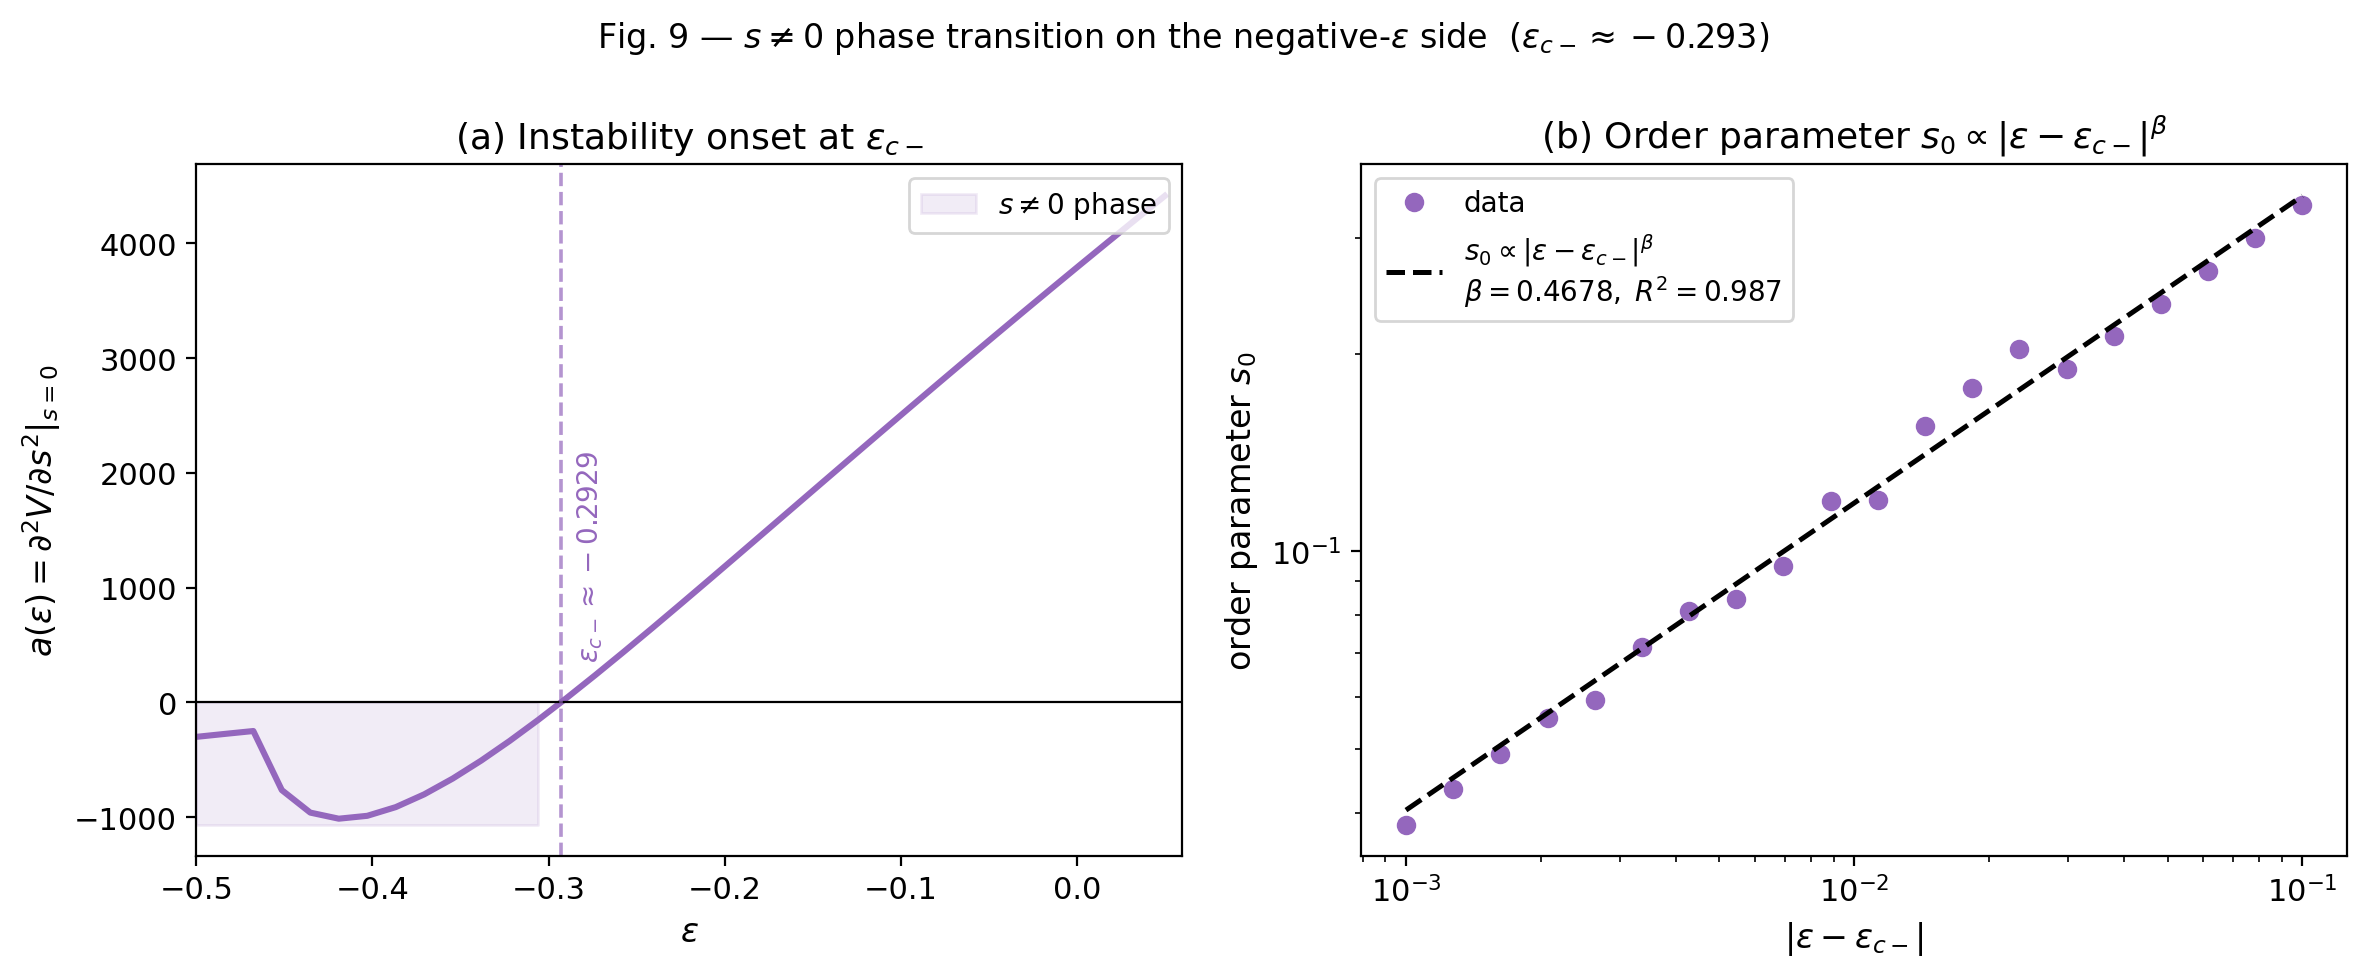
\includegraphics[width=0.85\textwidth]{figures/fig09_sneg_phase.png}
  \caption{Phase structure on the negative-$\varepsilon$ side.  The order
           parameter $s_0(\varepsilon)$ emerges continuously at
           $\varepsilon_{c-}=1/\!\sqrt{2}-1\approx -0.293$, consistent with a
           second-order transition into the $s\neq 0$ phase.}
  \label{fig:sneg_phase}
\end{figure}

\subsection{Geometric Interpretation}

In the $s\neq 0$ vacuum, $\mu_s^2$ becomes soft near the transition and then
returns to positive values, while $\mu_\varepsilon^2$ remains large and positive
over a wide range.  Furthermore, the $\phi$ direction is a pseudo-Goldstone
rather than an exact Goldstone, reflecting that $SO(2)$ is explicitly broken in
the $s\neq 0$ background.

The final picture of the spin-2 sector is summarised as follows.
\begin{enumerate}
  \item The full shear 5-plet is five-fold degenerate at $\mu_q^2=48\pi^2$ at
        the isotropic point.
  \item The first unstable direction on the positive side is the $m=0$ singlet
        $T_1$.
  \item On the negative side the $m=\pm 2$ sector governs the second-order
        transition into the $s\neq 0$ phase.
\end{enumerate}
This phase diagram plays the central role of the spin-2 block in the Landau-EFT
description of \S\ref{sec:eft}.
